\documentclass[letterpaper,11pt]{article}

\usepackage{graphics,graphicx, amsmath, amssymb,xcolor}
\usepackage{txfonts}
\usepackage{balance}
\usepackage[sort&compress]{natbib}
\usepackage{hyperref}

\setlength{\textwidth}{6.5in} 
\setlength{\textheight}{9in}
\setlength{\topmargin}{-0.0625in} 
\setlength{\oddsidemargin}{0in}
\setlength{\evensidemargin}{0in} 
\setlength{\headheight}{0in}
\setlength{\headsep}{0in} 
\setlength{\hoffset}{0in}
\setlength{\voffset}{0in}

%\makeatletter
%\renewcommand{\section}{\@startsection%
%{section}{1}{0mm}{-\baselineskip}%
%{0.5\baselineskip}{\normalfont\bfseries}}%
%\makeatother

\newcommand{\no}{\noindent}
\newcommand{\comment}[1]{{\color{red}\bf{(#1)}}}

\def\apj{ApJ}
\def\apjl{ApJ}
\def\mnras{MNRAS}
\def\pasj{PASJ}
\def\aap{A\&A}
\def\prd{Phys. Rev. D.}
\def\araa{ARAA}
\def\nat{Nature}

\begin{document}
\pagestyle{plain}
\pagenumbering{arabic}

\begin{center} 
\Large\bfseries{Code Performance and Scaling Tests}
\end{center}

\section{Code}

The simulation code we are using is the Adaptive Refinement Tree ({\tt ART}) code \citep{kra99,kra02, rudd_etal08}.  {\tt ART} is a fully MPI/OpenMP parallel $N$-body/hydrodynamic code, which uses adaptive mesh refinement (AMR) to achieve high dynamic range. It models the evolution of dark matter and the baryonic components such as gas and stars in the live cosmological setting. The {\tt ART}'s hydrodynamic solver is based on the Eulerian mesh technique which is especially good at capturing shocks, turbulent mixing, and fluid instabilities which are crucial for modeling the interactions between the outflows from AGN feedback and the surrounding cluster gas. The current {\tt ART} code is equipped with baryonic physics modules, including realistic metal-dependent radiative gas cooling, UV radiation background, star formation, and energy feedback from Supernovae Ia and II.  

{\tt ART} achieves load balancing using domain decomposition of the computational box. The box is divided into uniform grids (with $2^N$ number of grid cells on each side). We then use space-filling curve (SFC) to map the 3D coordinates of each cell into a 1D vector. Load-balancing of the simulation is achieved when the SFC is divided among the MPI tasks, where each MPI task is responsible for approximately equal amount of number of particles and hydro cells, thus making sure that each MPI load is approximately the same. As the simulation progresses, the load for each MPI task is re-adjusted for every 5 time steps to ensure each task have similar amount of load. For each MPI task, the load is shared among OpenMP threads where the code can be parallelized (e.g., for-loops). 

\section{Performance and Scaling Tests}

\subsection{Test Simulation}
We tested the performance of our code on Stampede2 with the lowest resolution LR run of the proposed simulation. The box size of the simulation is $50\,h^{-1}$~Mpc on the side, with $256^3$ root grid and effective number of particles of $1024^3$. The maximum level of mesh refinement is 8, corresponding to the spatial resolution of $0.76\,h^{-1}$~kpc. The test simulation we are using has an effective resolution of $N_p = 1024^3$, which requires memory of at least 2 SKX nodes ($2\times 192 = 384$~GB). Here we test our simulation with 4 SKX nodes. 

\subsection{KNL nodes versus SKX nodes}

We tested our code on both Knights Landing (KNL) and Skylake (SKX) nodes on Stampede2. We have found that SKX nodes out-performs KNL nodes by a factor of $4-5$. This is due to the fact that our code is more optimized for MPI parallelization than OpenMP parallelization and vectorization, thus the large number of cores per node in KNL offer no advantages over SKX. SKX also has high clock speed than KNL. For the rest of the tests, we focus exclusively on testing SKX nodes. 

\subsection{Number of MPI tasks versus OpenMP threads}

\begin{figure}[htbp]
\centering
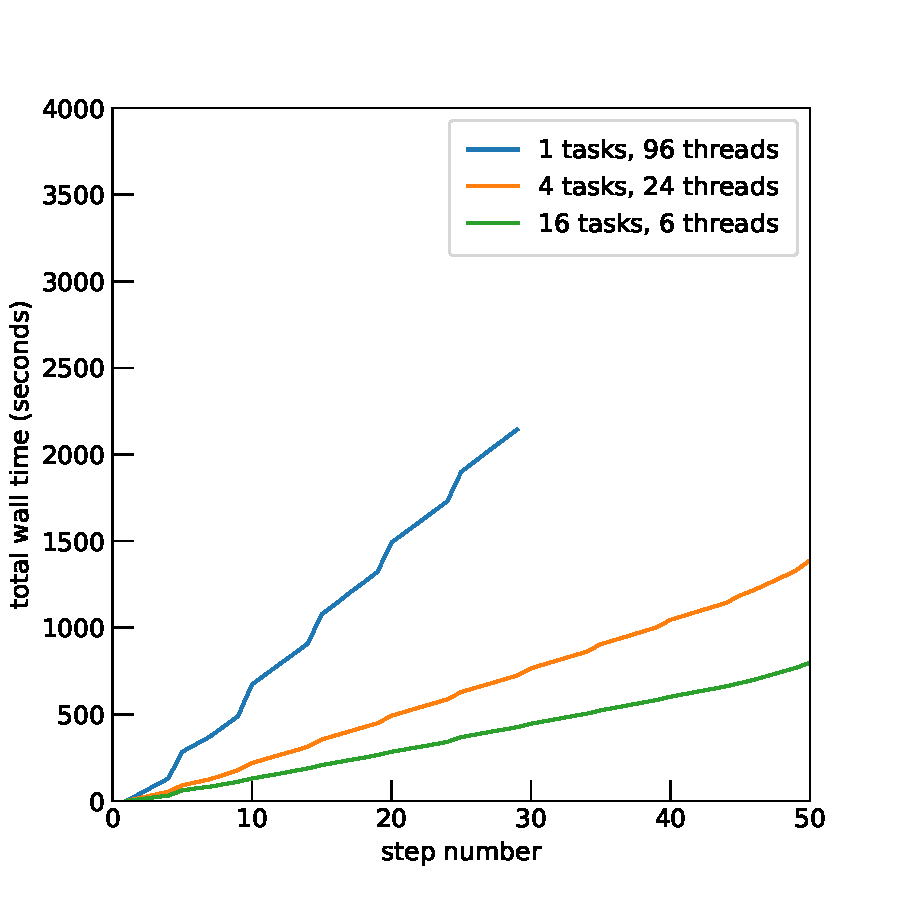
\includegraphics[width=0.32\textwidth]{cum_time_step_N4.pdf}
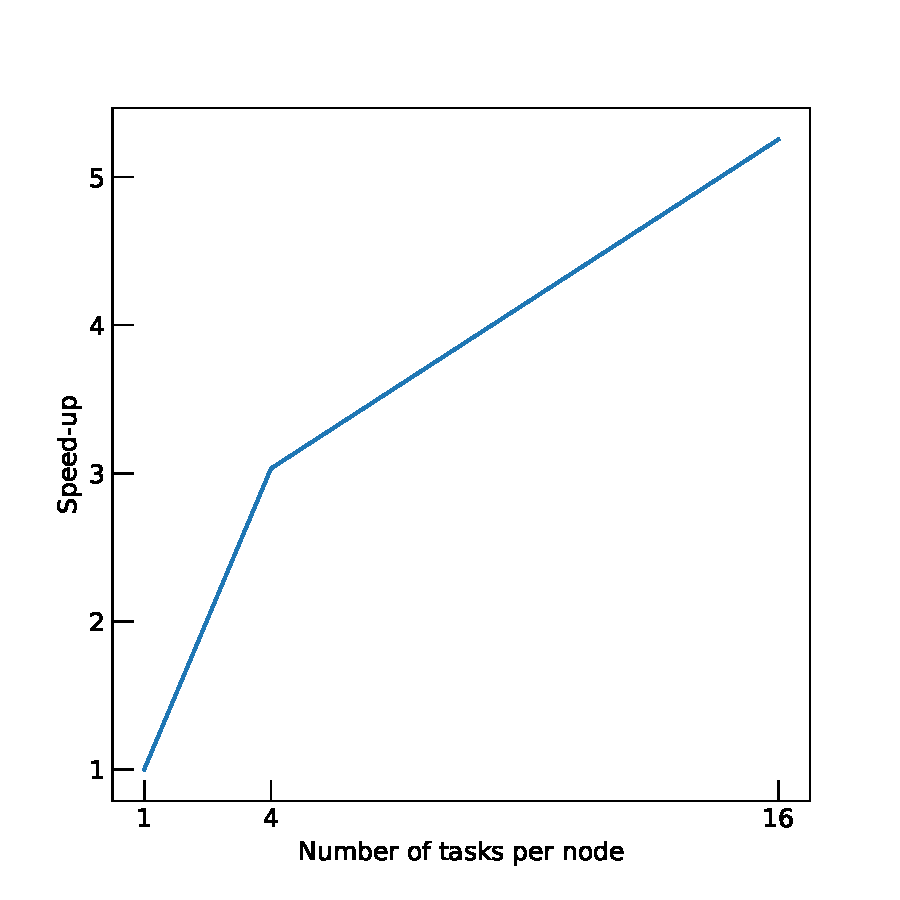
\includegraphics[width=0.32\textwidth]{task2thread_N4.pdf}
\caption{{\em Left}: Total wall time of the test L50 runs with AGN feedback for different ratios of MPI tasks per node and OpenMP threads per task, plotted as a function of the time steps of the simulation. The runs are performed on 4 SKX nodes in Stampede2. {\em Right}: speed-up as a function of the number of MPI tasks per node.   
}  
\label{fig:mpi_omp}
\end{figure}

Figure~\ref{fig:mpi_omp} shows the total wall time versus the simulation steps of our test simulations for 4 SKX nodes. The number of MPI tasks and the number of OpenMP threads for each task is varied, while keeping the total number of OpenMP threads fixed to the total number of physical threads available on each SKX node $= 96$. As the ratio of MPI tasks to OpenMP threads increase, the code performance increase quite significantly. With 16 MPI tasks/6 threads per task the speed-up is 5 times over a single MPI task with full 96 threads per task. Increasing the number of MPI task per node beyond 16 is not practical since the memory available for each MPI task (12 GB for Skylake) is not enough to run our simulation. Thus, the optimal MPI task per node is 16, corresponding to 6 OpenMP threads per task. 

\begin{figure}[htbp]
\centering
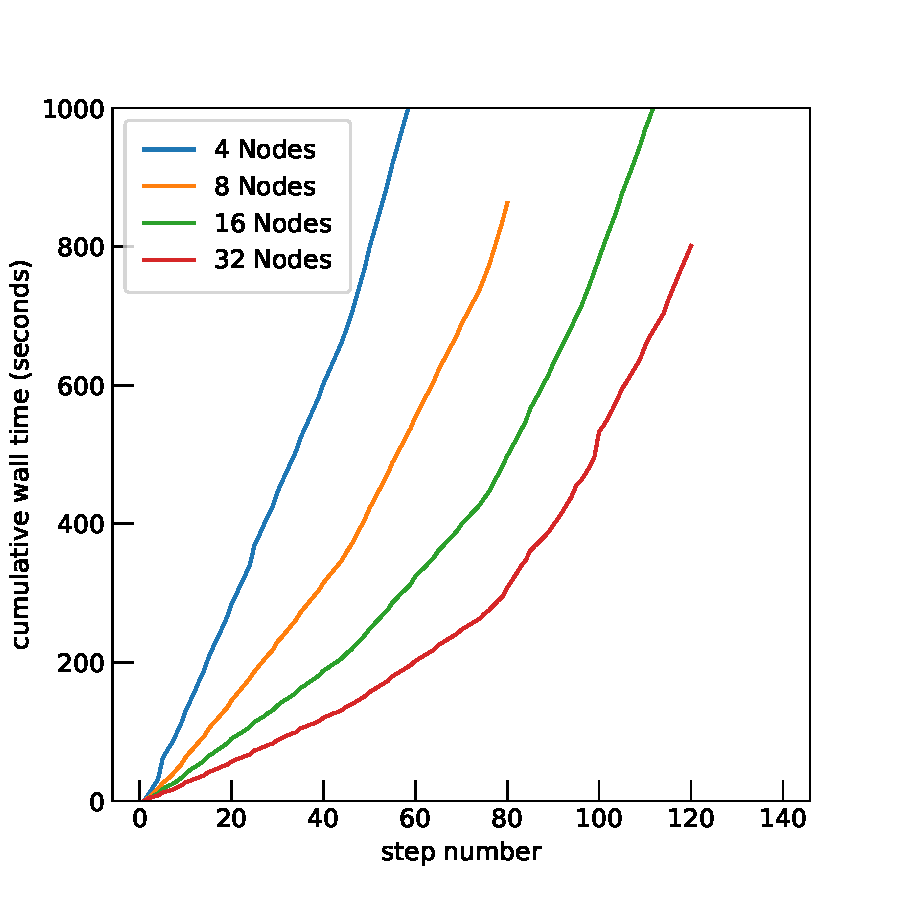
\includegraphics[width=0.32\textwidth]{cum_time_6.pdf}
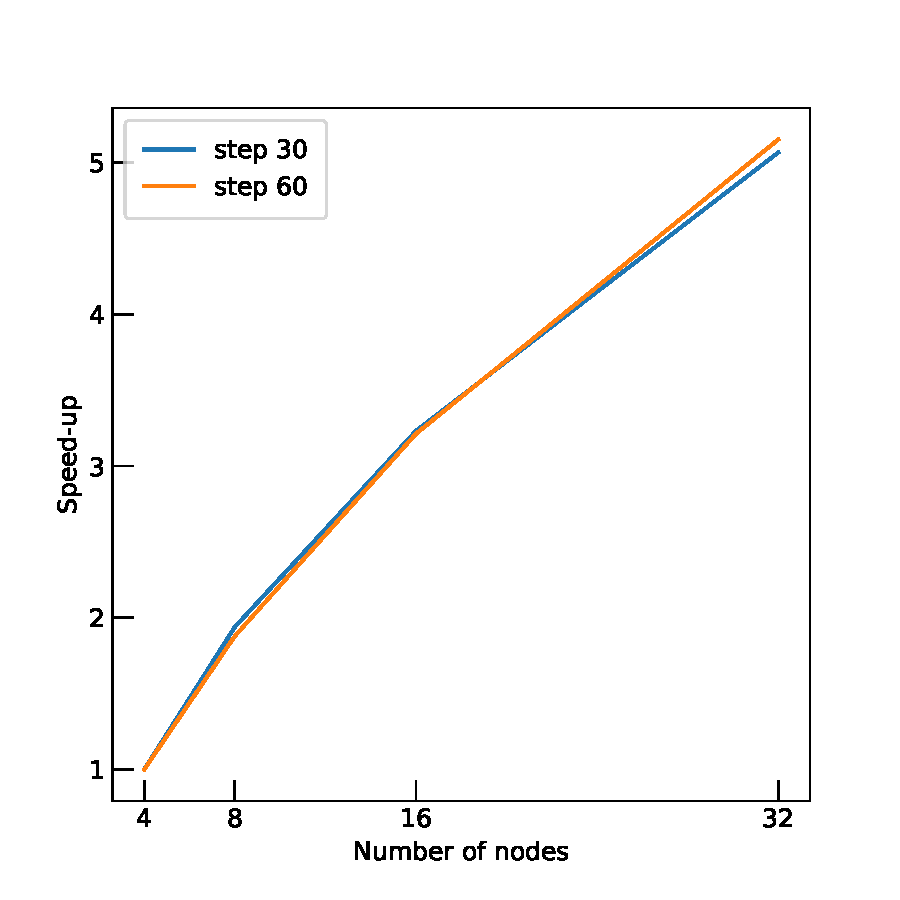
\includegraphics[width=0.32\textwidth]{strong_scaling_6.pdf}
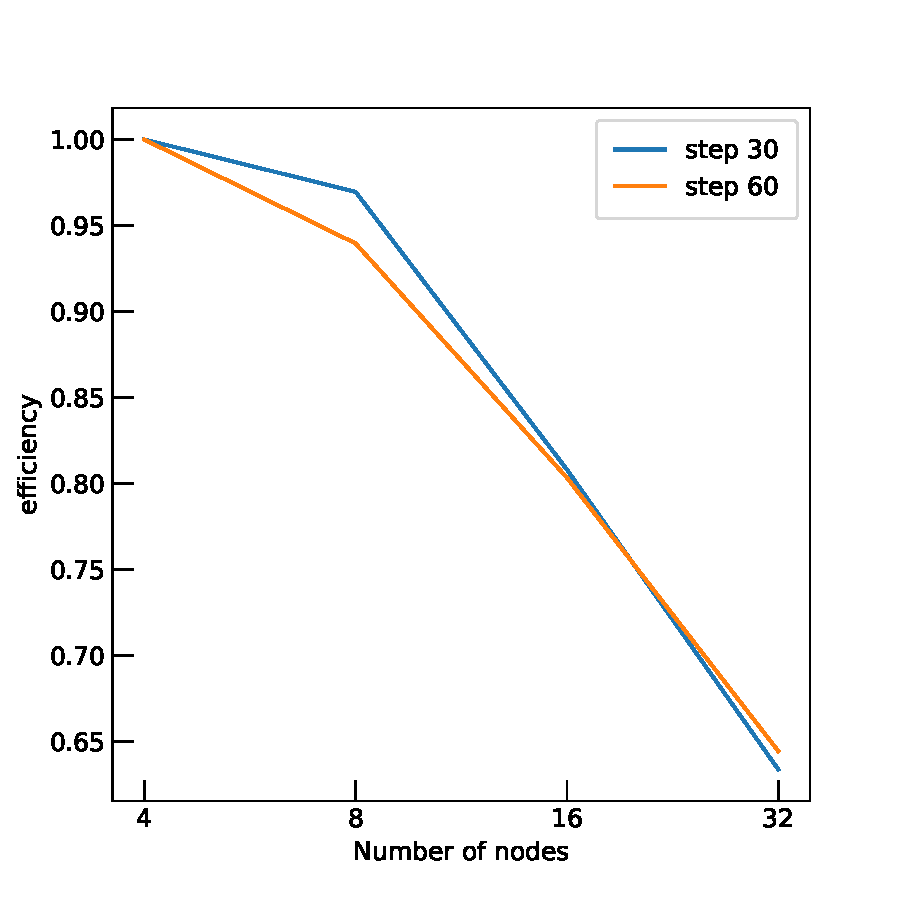
\includegraphics[width=0.32\textwidth]{strong_scaling_efficiency_6.pdf}

\caption{{\em Left}: Wall time taken for the test simulation with different number of nodes, as a function of the simulation step. {\em Middle}: Speed-up of the test L50 runs with AGN feedback when the number of nodes are increased. The speed-up here is defined as the ratio of the wall time of the runs for 4 nodes to the wall time taken for other number of nodes. The wall time is measured at time steps 30 (blue lines) and 60 (orange lines) for each run, with 16 MPI tasks per node and 6 OpenMP threads per MPI task. {\em Right}: Efficiency of the runs as at function of number of nodes. 
All runs are performed with 16 tasks per node and 6 threads per task. 
}  
\label{fig:strong_scaling}
\end{figure}

\subsection{Strong Scaling}

Figure~\ref{fig:strong_scaling} shows the strong scaling of our code. Using the optimal MPI-to-OpenMP ratio (16 tasks per node, 6 threads per task), we increase the number of SKX nodes for our test simulation from 4 to 8, 16, and 32.
It demonstrates that our code scales quite well with up to 16 nodes. This is shown more clearly when we plot the speed-up and efficiency against the number of nodes. The speed-up at 16 nodes is around a factor of $3.2$, and retains an efficiency of $80\%$. At 32 nodes, the efficiency drops to $60\%$. The result is insensitive to the computing step. The speed-up is nearly identical for computing step number 30 and 60. Adding more nodes do not improve the performance significantly further due to the increase in communication overhead between nodes.  

\subsection{Weak Scaling}

\begin{figure}[htbp]
\centering
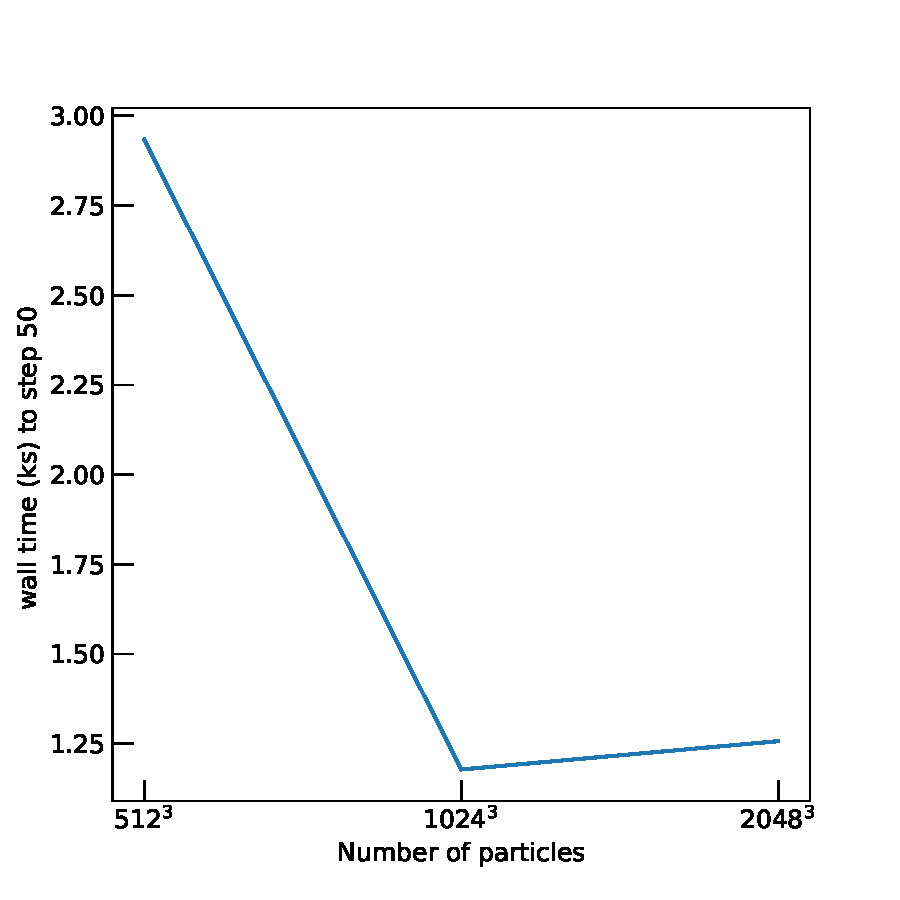
\includegraphics[width=0.4\textwidth]{weak_scaling.pdf}

\caption{Wall time taken for the test simulation as a function of the effective number or particles of the simulations (i.e., resolution), The number of particles per core is fixed for all three simulation runs. 
}  
\label{fig:weak_scaling}
\end{figure}

Here we demonstrate how our code scales with increasing simulation size. Figure~\ref{fig:weak_scaling} shows the wall time of the test simulation with different effective number of at particles $N_P$ which determines the numerical resolution of the simulation. The particles per core is kept fixed at $5.6\times 10^6$ for all three simulation. The figure shows quite good weak scaling. The wall time drops quite sharply from $N_p = 512^3$ to $1024^3$, and shows $\sim 10\%$ increase from $N_p = 1024^3$ to $2048^3$. We expect the wall time will only increase slightly by a similar amount for the resolution of our proposed high resolution production run with $N_p = 4096^3$. 

\subsection{Increase in Time Step }
\begin{figure*}
\centering
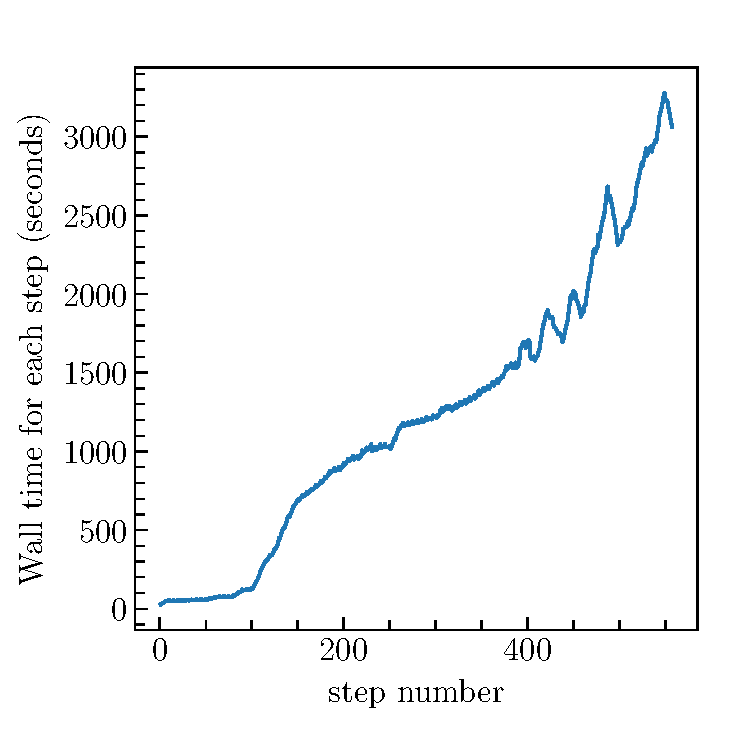
\includegraphics[width=0.5\textwidth]{code/plot_step.pdf}
%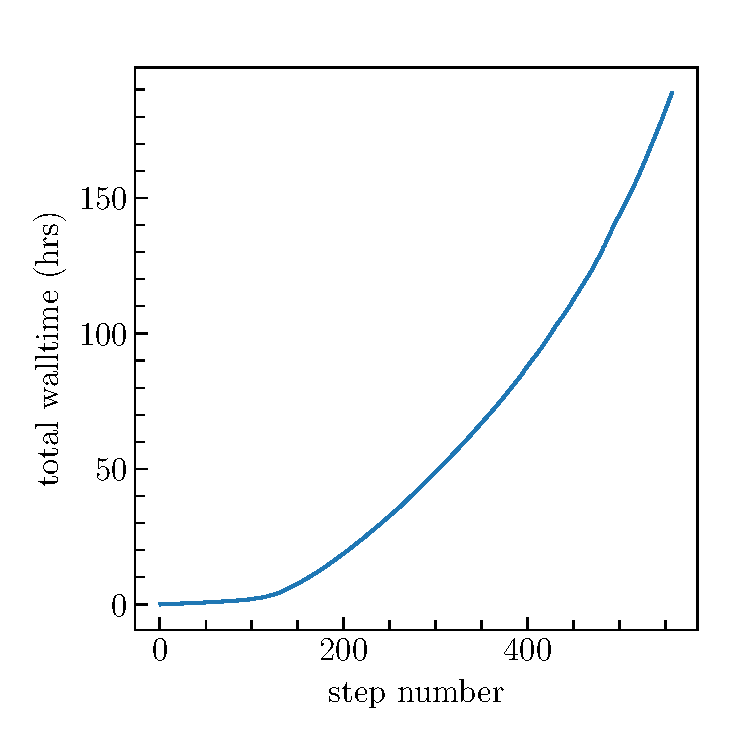
\includegraphics[width=0.35\textwidth]{code/plot_totalstep.pdf}
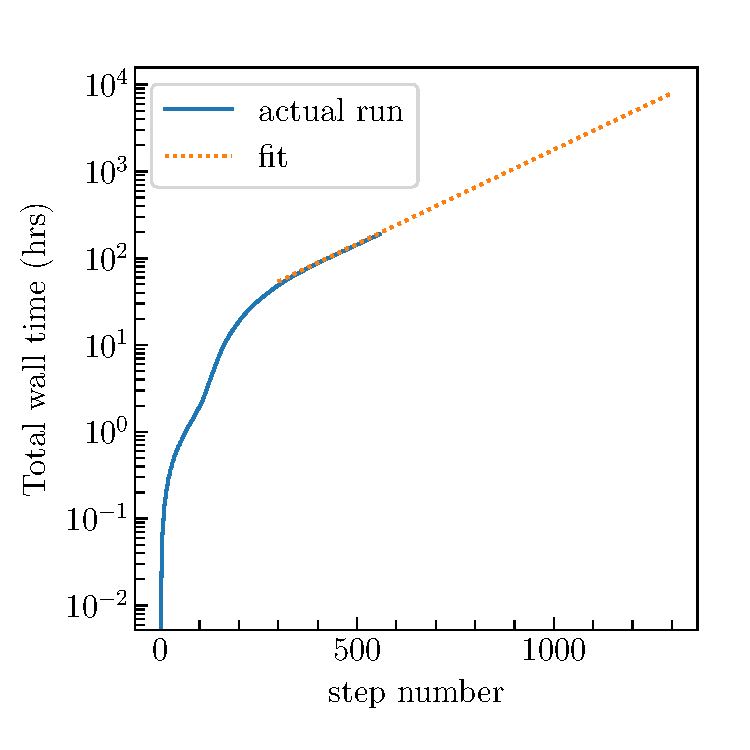
\includegraphics[width=0.5\textwidth]{code/plot_totalstep_fit.pdf}
\caption{Top: Wall time taken for each time step as a function of time step. Bottom: Total wall time as a function of time step. The orange dotted line marks the extrapolation of the total wall time from a fit to the actual walltime (for time steps $> 300$). 
}  
\label{fig:step}
\end{figure*}
As the simulation proceed, the hydro cell and inter-particle separations decrease, resulting in the increase the load in both hydro solver and gravity solver, thus, the wall time taken for each time step increases. We estimate the increase in wall time as a funciton of time step for $N_p=1024^3$ run ( with 4 MPI tasks and 48 OpenMP thread for each task).  Shown in the top panel of Figure~\ref{fig:step}, the wall time increases rapidly from around 50 seconds to 1000 seconds from time step 100 to 200 time. The wall time then increases steadily from 1000 seconds to 3000 seconds from time step number 200 to 550.
%with an average increase of 5 seconds per time step. 
%The estimated total time steps for a single run is around 1200. Extrapolating the current result, the estimated increase in wall time for each time step is around 3700 seconds. 

As wall time taken for individual time step increases, the {\em total} wall time, i.e., cumulative wall time at each time step, increases accordingly. Shown in the bottom panel of Figure~\ref{fig:step}, the total wall time increases from 0.7 hrs to 20 hrs from time step 50 to 200. The  increase in wall time becomes exponential from time step 200 onward, reaching 150 hrs at around time step 500. We have fitted the total wall time dependence as an exponential function (shown as orange dotted line). Extrapolating the fitted function to timestep 1300 where the simulation is expected to finish , the estimated total wall time is around $10^4$ hours. 

\bibliographystyle{apj}
\bibliography{references}

\end{document}